% !TeX root = Bericht_main.tex


	
\begin{figure}[H]
	\centering
	\captionabove{rkorder = 4, Problem = Riemann, Finite Volumen,
	Energie}
	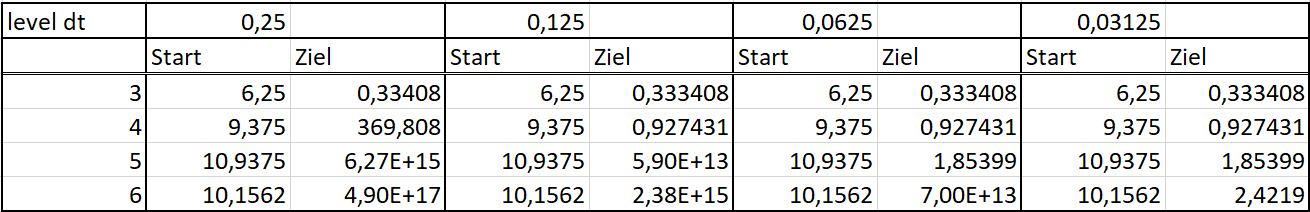
\includegraphics[width=\textwidth]{../Aufgabe21/rkorder4RiemannEnergieTabelle.png}
	
\end{figure}

\begin{figure}[H]
	\centering
	\captionabove{rkorder = -2, Problem = Riemann, Finite Volumen,
	Energie}
	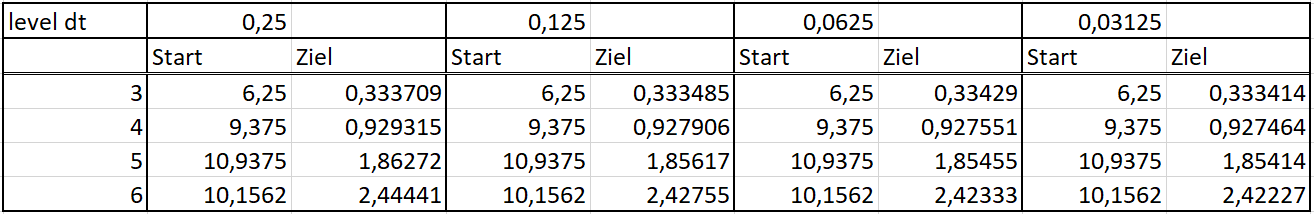
\includegraphics[width=\textwidth]{../Aufgabe21/rkorder-2RiemannEnergieTabelle.png}
	
\end{figure}

\begin{figure}[H]
	\centering
	\captionabove{deg = 0, Problem = CircleWave, Finite Volumen,
	Energie}
	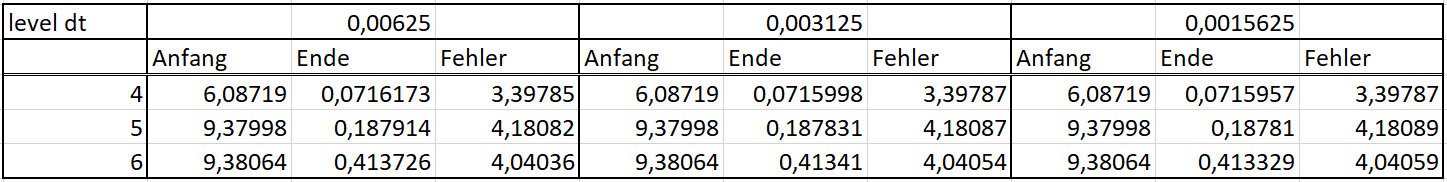
\includegraphics[width=\textwidth]{../Aufgabe21/deg=0CircleWaveEnergieTabelle.png}
	
\end{figure}

\begin{figure}[H]
	\centering
	\captionabove{deg = 2, Problem = Riemann, Discontinuous Galerkin,
	Energie}
	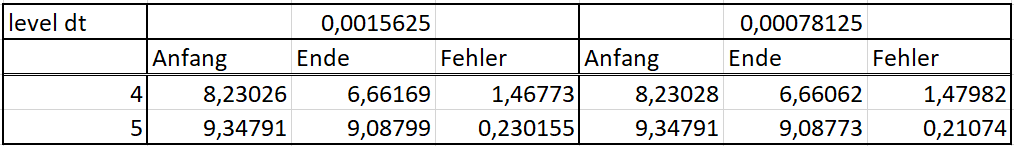
\includegraphics[width=\textwidth]{../Aufgabe21/deg=2CircleWaveEnergieTabelle.png}
	
\end{figure}